% Owner: chm. Conditional Q3 answer using pinned CYJ v8 and Q1 v2.
% Evidence: outputs/Q3/curated_manifest.json and pinned upstream manifest.
\subsection{算力约束下的条件配置与结构转移}
\label{sec:q3_numerical}

\subsubsection{题面成本、输入范围与配比策略}
题面要求在参数量 $N$、训练数据量 $D$、数据质量 $Q$ 与领域配比
$\boldsymbol p$ 间配置有限算力，并将上下文长度 $L_c$ 作为外生情景。
本文以十亿参数、十亿 Token 为 $N,D$ 的单位，按题面三项代理成本计算
\begin{equation}
\begin{aligned}
C(N,D,Q;L_c)&=C_{\rm train}+C_{\rm quality}+C_{\rm attention},\\
C_{\rm train}&=6\times10^{18}ND,\\
C_{\rm quality}&=10^9D\max\{g(Q)-g(Q_0),0\},\\
C_{\rm attention}&=2\times10^{14}L_cND.
\end{aligned}
\label{eq:q3_cost_v8}
\end{equation}
其中 $g$ 分别取题面附录 B 的指数、幂函数与对数渐进形式；
$Q_0=0.5$ 是明确给定的质量基线情景，不是跨附件估计值。
附件 C7 支持 $L_c=2048,8192,131072$ Token 的外生对照，高端情景样本较少。
题面建议的预算为 $10^{19},10^{22},10^{24}$ FLOPs；另以 $10^{20}$ 作过渡诊断。

预测器固定为 cyj 的 \texttt{cyj.ndqp.scenario.v8}：B1 五参数 $N$--$D$ 主干
和 B7 三参数质量增量在各自来源中拟合，配比效应消费第一问冻结的
\texttt{chm.q1.v2.0}。在主情景中，$Q=\phi(Q_A(\boldsymbol p))$
由六个已映射 A1 质量域给出单调质量代理，联合 Loss 写为
\begin{equation}
\begin{aligned}
\widetilde L_8(N,D,\boldsymbol p)
={}&\Bigl[E+AN^{-\alpha}+BD^{-\beta}\\
&+\bigl(1-\phi(Q_A(\boldsymbol p))\bigr)
\bigl(G_0+G_N\log N+G_D\log(D/100)\bigr)\Bigr]\\
&\hspace{2em}\times\exp\{r_w(\boldsymbol p)\}.
\end{aligned}
\label{eq:q3_v8_loss}
\end{equation}
这里 $r_w$ 是 A 侧 13 个目标域等权的相对配比响应。
$\phi$ 与指数幅度是明示的\emph{未标定跨源假设}，
并无 A/B 成对训练实验识别它们或区分质量与配比的重叠贡献。
本问主表只作该假设下的条件资源配置，不解释为真实训练 Loss 的保证值。

为使 CYJ 第二问的正式理论与本问独立可核，记 $\mathcal M$ 为第一问
有 A1 质量评分且映射到 A4 配比坐标的六个训练域，定义
\begin{equation}
\begin{aligned}
Q_A(\boldsymbol p)&=
\frac{\sum_{i\in\mathcal M}p_iq_{A,i}}{\sum_{i\in\mathcal M}p_i},\\
\phi(Q_A)&=\operatorname{clip}_{[0.1,1]}
\left[0.1+0.9\frac{Q_A-q_{\min}}{q_{\max}-q_{\min}}\right],\\
r_w(\boldsymbol p)&=\sum_{k=1}^{13}w_k
\frac{\widehat L_{A,k}(\boldsymbol p)-
\widehat L_{A,k}(\boldsymbol p_{\rm ref})}
{\widehat L_{A,k}(\boldsymbol p_{\rm ref})},\quad w_k=1/13.
\end{aligned}
\label{eq:q3_v8_bridges}
\end{equation}
无映射域的评分保持缺失，不以零代入；映射质量覆盖为零时拒绝预测。
Q1 的 $\widehat L_{A,k}$ 是冻结二阶交互面，$r_w$ 在参考配比为零。
第二问 B1 主干与 B7 半合成质量增量的冻结参数为
\begin{equation*}
\begin{aligned}
E&=1.689838,& A&=0.353969,& B&=1.240275,\\
\alpha&=0.339985,&\beta&=0.279892,\\
G_0&=0.371703,&G_N&=-0.061115,&G_D&=-0.014961.
\end{aligned}
\end{equation*}
这些参数在 B1/B7 各自来源内估计；$\phi$ 的斜率与
$\exp\{r_w\}$ 的跨来源幅度是可检验的建模假设。

题面允许配比由前两问确定。固定策略采用第二问 v8 已发布的
A4 已观测配方 172，它满足第一问 \texttt{direct+near} 质量政策，
代理质量为 $0.67136\ge Q_0$。
第一问无约束等权主配方的同一代理质量约为 $0.38578$，
不满足本节的 $Q\ge Q_0$ 约束，因此没有被暗中代入主表。
作为配比可调的条件方案，另对同时满足质量政策与 $Q\ge Q_0$ 的 87 个 A4
已观测配方逐一寻优；有限候选枚举不等于连续配比凸包全局最优。
该配方表来自 RegMix 作者公开实验\cite{regmix2025}，不是另一次独立外测。
所有模式采用 v8 的共同支持域
$N\in[0.070542,11.965825]$、$D\in[10,299.893]$、$Q\in[0.1,1]$。

\subsubsection{求解方法与预算可行性}
固定配方使 $Q$ 与 $r_w$ 固定。记
$c(L_c)=6\times10^{18}+2\times10^{14}L_c$、
$h(Q)=10^9\max\{g(Q)-g(Q_0),0\}$。当前 v8 参数在声明支持域内
满足 $\partial\widetilde L_8/\partial D<0$，故给定 $N$ 时
\begin{equation}
D^*(N)=\min\left\{D_{\max},\frac{C_{\max}}{c(L_c)N+h(Q)}\right\},
\qquad
C_{\min}=D_{\min}\{c(L_c)N_{\min}+h(Q)\}.
\label{eq:q3_v8_reduction}
\end{equation}
若 $C_{\max}<C_{\min}$，直接报告支持域内不可行。
当前拟合系数满足 $A,B,\alpha,\beta>0$、$G_N,G_D\le0$，
质量收益在矩形支持域内为正；据此检查分段目标对 $\log N$ 的凸性，
用导数二分并核对成本和边界。联立有限配方解对每个候选重复上述二维求解，
选择条件 Loss 最低者。与此并列的\emph{独立质量投入方案}固定配方 172，
把 B7 原生半合成坐标 $Q_B\in[Q_0,1]$ 视为可投入的工程控制量，
用题面 $g(Q_B)$ 计费，并在共同支持域内联立选择 $N,D,Q_B$。
两种方案分别回答“通过配比改变质量代理”与“给定配比，额外处理数据是否值得投入”；
后者要求质量处理确能移动 B7 坐标这一可检验假设，目前不是已观测干预。
两种输入机制的 Loss 差不能直接解释为因果增益。

CYJ 的理论边际条件在本问按变量角色使用。固定配比时，
$\partial\widetilde L_8/\partial N$ 与
$\partial\widetilde L_8/\partial D$ 均为负；当 $Q>Q_0$ 时，
$C_N=c(L_c)D$、$C_D=c(L_c)N+h(Q)$、
$C_Q=10^9Dg'(Q)$。只有变量可独立微调、解为内点且预算激活时，
才可比较单位成本的边际 Loss 改善。主模型的 $Q$ 随 $\boldsymbol p$
变化，故配比方向导数须同时包含
$-\exp\{r_w\}G\nabla_{\boldsymbol p}\phi$ 与
$\widetilde L_8\nabla_{\boldsymbol p}r_w$；质量成本也随配比改变。
本问实际对已观测配方作有限枚举，不把连续 KKT 条件误作离散全局证明。

表\ref{tab:q3_v8_power}是幂函数质量成本下的有限配方联立结果。
预算 $10^{19}$、131072 Token 的三类成本均不足以进入 v8 声明支持域；
幂函数场景在另外两个上下文改选低质量成本的配方 477 才可行。
\begin{table}[htbp]
\centering\small
\caption{幂函数质量成本下的 v8 条件资源配置；$N,D$ 为十亿单位，Loss 为未标定情景值}
\label{tab:q3_v8_power}
\begin{tabular}{rrrrrrr}
\toprule
预算/FLOPs & $L_c$ & 配方 & $N$ & $D$ & $Q$ 代理 & 条件 Loss\\
\midrule
$10^{19}$ & 2048 & 477 & 0.104 & 10.000 & 0.600 & 3.1551\\
$10^{19}$ & 8192 & 477 & 0.087 & 10.000 & 0.600 & 3.2038\\
$10^{19}$ & 131072 & \multicolumn{5}{c}{支持域内不可行}\\
$10^{22}$ & 2048 & 172 & 7.291 & 210.799 & 0.671 & 2.0809\\
$10^{22}$ & 8192 & 172 & 6.661 & 193.874 & 0.671 & 2.0944\\
$10^{22}$ & 131072 & 172 & 3.214 & 95.943 & 0.671 & 2.2179\\
$10^{24}$ & 2048 & 172 & 11.966 & 299.893 & 0.671 & 2.0195\\
$10^{24}$ & 8192 & 172 & 11.966 & 299.893 & 0.671 & 2.0195\\
$10^{24}$ & 131072 & 172 & 11.966 & 299.893 & 0.671 & 2.0195\\
\bottomrule
\end{tabular}
\end{table}

固定配方 172 的 36 个主网格情景中 30 个可行；有限配方联立后 33 个可行。
例如 $10^{19}$、2048 Token 的幂函数成本使配方 172 的最小成本
约为 $1.1554\times10^{19}$ FLOPs，故其不可行；配方 477 可行。
在 $10^{19}$、8192 Token 下，幂函数和对数函数同样需要改选配方 477，
而指数函数可保持 172。到 $10^{22}$、8192 Token 时，三类成本都选择 172，
其 $(N,D)$ 分别约为 $(6.599,196.983)$、$(6.661,193.874)$、
$(6.625,195.681)$，条件 Loss 为 $2.09389,2.09442,2.09411$。
在 $10^{24}$ 时达到 v8 的 $N,D$ 支持上界，8192 Token 幂成本仅使用
约 $2.76\%$ 的预算；这说明当前模型不支持继续外推资源收益。

独立质量投入方案的 36 格中有 33 格可行。表\ref{tab:q3_native_quality}
把 8192 Token、幂成本下的四个量级放在同一决策轴上：
\begin{table}[htbp]\centering\small
\caption{固定配方 172、可独立投入 $Q_B$ 的条件最优；$N,D$ 为十亿单位}
\label{tab:q3_native_quality}
\begin{tabular}{rrrrrl}\toprule
预算/FLOPs & $N$ & $D$ & $Q_B$ & 条件 Loss & 活跃约束\\\midrule
$10^{19}$ & 0.1309 & 10.000 & 0.500 & 3.0969 & $D_{\min},Q_0$,预算\\
$10^{20}$ & 0.7628 & 10.000 & 0.973 & 2.5618 & $D_{\min}$,预算\\
$10^{22}$ & 5.2587 & 222.936 & 1.000 & 2.0232 & $Q_{\max}$,预算\\
$10^{24}$ & 11.9658 & 299.893 & 1.000 & 1.9570 & $N_{\max},D_{\max},Q_{\max}$\\
\bottomrule\end{tabular}
\end{table}
低预算先守住 $D=10$ 的训练下限，质量停在基线 $Q_0$；
$10^{20}$ 的过渡预算已可把质量代理升至 0.973，数据量仍在下限；
$10^{22}$ 时值得在该假设下把质量升到 1，同时扩展 $N,D$。
配比联立方案在 $10^{19}$、8192 Token 的幂成本下改选配方 477，
到 $10^{22}$ 回到 172；它与独立质量投入的优劣需先确定实际可操作的质量机制。
表中全部是半合成质量曲线与未标定配比桥下的模型内条件解。

最高预算时，配比联立方案 8192 Token 幂成本实际只需
$2.7621\times10^{22}$ FLOPs（预算的 $2.76\%$），
独立质量方案只需 $2.8816\times10^{22}$（$2.88\%$）。
其余预算\emph{超出本模型已声明的 $N,D,Q$ 支持域}；
相同的上界解不表示现实继续训练没有收益。
若确需使用 $10^{24}$，应先取得更大 $N,D$ 的可比训练与验证数据，
再扩大模型支持域后重新优化；在此之前只报告受限解，并把剩余资源保留为未分配。

\subsubsection{结构转移与上下文敏感性}
对预算 $B$ 定义稳定配置状态
\begin{equation}
S(B)=\bigl(\mathbf 1_{\rm feasible},\operatorname{index}(\boldsymbol p^*(B)),
\mathcal A_{N,D,B}(B)\bigr),
\label{eq:q3_v8_state}
\end{equation}
其中 $\mathcal A$ 为参数、数据与预算约束的活跃集。
若一个预算附近的左右稳定状态不同，则称发生本模型的数值结构转移；
成本占比的连续变化本身不算结构转移。
每个 C7 上下文与成本族在 $10^{19}$--$10^{24}$ FLOPs 扫描 161 个对数点，
对异状态相邻点二分至预算相对宽度小于 $10^{-4}$。
固定策略记录 33 个、已观测配方联立记录 49 个括区；
包含支持域可行性开启、配方切换以及 $D_{\min}$、$D_{\max}$、
$N_{\max}$ 和预算约束的切换。
例如 8192 Token、幂成本的配方 $477\to172$ 切换位于
$[1.610535,1.610648]\times10^{19}$ FLOPs。
131072 Token 的三个成本族在可行性边缘还依次出现多个短暂配方状态，
81 点粗网格漏掉其中一些，因此不声称更窄的状态已穷尽。
这些是给定半合成模型、成本代理与数值容差的转移，
不是现实大模型训练的精确相变阈值。

\begin{figure}[htbp]
\centering
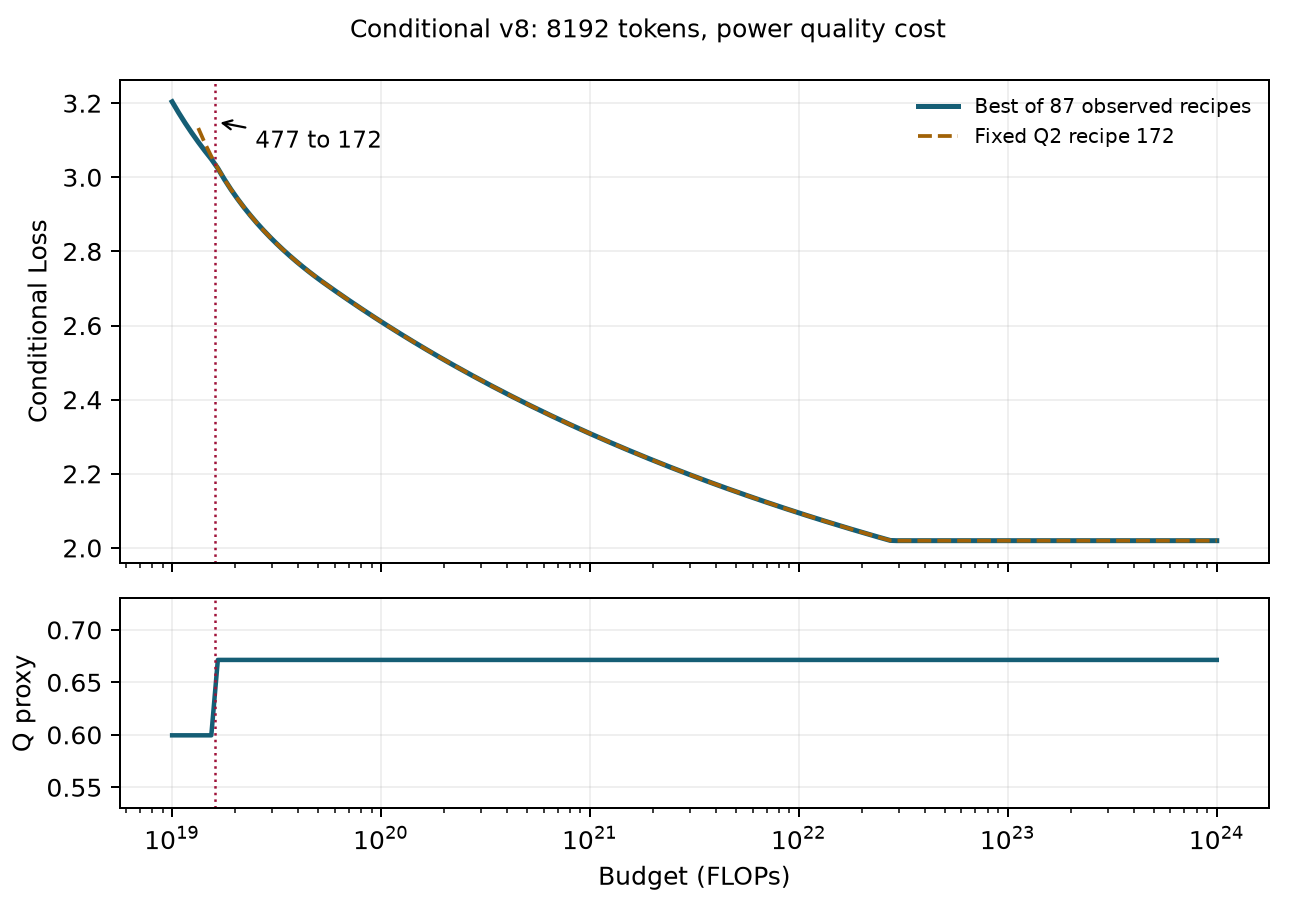
\includegraphics[width=0.86\textwidth]{figures/Q3/q3_v8_power_8192.png}
\caption{8192 Token、幂函数质量成本下的条件 Loss 与配比质量代理。
纵虚线是已观测候选中配方 $477\to172$ 的数值切换括区；
曲线只在 v8 共同支持域内绘制。}
\label{fig:q3_v8_budget}
\end{figure}

注意力与基础训练开销的比值由题面公式直接消去 $N,D$：
\begin{equation}
\frac{C_{\rm attention}}{C_{\rm train}}=\frac{L_c}{30000},
\qquad L_{\rm crit}=30000\ {\rm Token}.
\label{eq:q3_v8_context}
\end{equation}
C7 的 2048、8192、131072 Token 分别给出约 0.0683、0.2731、4.3691。
$L_{\rm crit}$ 是两项简化成本相等的位置，不是观测得到的模型能力阈值；
尤其长上下文情景应按稀疏支持谨慎解释。

\subsubsection{跨源假设稳健性与公开实验检验}
围绕 v8 主情景逐次只改变一个未标定设定。质量基线取
$Q_0\in\{0.45,0.55,0.60,0.65\}$；质量映射绕冻结参考点改变斜率：
\begin{equation}
\phi_s(Q_A)=\operatorname{clip}_{[0.1,1]}
\left[q_{\rm ref}+s\frac{0.9}{q_{\max}-q_{\min}}
(Q_A-Q_A^{\rm ref})\right],\qquad s\in\{0.5,1.5\},
\end{equation}
其中 $Q_A^{\rm ref}=0.783104$、$q_{\rm ref}=0.435406$。
配比桥则改成 $\exp\{\lambda r_w\}$，检验 $\lambda=0,2$；
主情景为 $(Q_0,s,\lambda)=(0.5,1,1)$。这些点是明示压力情景，
不是参数置信区间。每次重算三档题面预算、三种质量成本和三个上下文，
并在 8192 Token、幂成本的 $10^{19}$--$10^{21}$ 预算段扫描配方转移。

\begin{table}[htbp]
\centering\small
\caption{单因素假设压力下的离散配方变化；变化格数相对于主情景的 27 个题面格，低/中列为 8192 Token 幂成本}
\label{tab:q3_v8_robustness}
\begin{tabular}{lrrrrr}
\toprule
情景 & 合格配方数 & 可行格数 & 变化格数 & 低预算配方 & 中预算配方\\
\midrule
主情景 & 87 & 24 & 0 & 477 & 172\\
$Q_0=0.45$ & 101 & 24 & 4 & 97 & 172\\
$Q_0=0.55$ & 82 & 24 & 2 & 477 & 172\\
$Q_0=0.60$ & 73 & 24 & 4 & 475 & 172\\
$Q_0=0.65$ & 60 & 24 & 4 & 172 & 172\\
$s=0.5$ & 79 & 24 & 4 & 172 & 172\\
$s=1.5$ & 93 & 24 & 9 & 97 & 172\\
$\lambda=0$ & 87 & 24 & 24 & 159 & 88\\
$\lambda=2$ & 87 & 24 & 1 & 477 & 172\\
\bottomrule
\end{tabular}
\end{table}

主情景的 $Q_{477}=0.599515$；提高 $Q_0$ 至 0.60 后配方 477
不再合格，低预算改选 475；至 0.65 改选 172。质量映射斜率取
1.5 倍时，低预算改选 97，且 $10^{22}$ FLOPs 的 131072 Token
三个成本族也换配方。令 $\lambda=0$ 则所有 24 个可行题面格的
最佳配方均变化，说明主方案配比结论对跨源桥强度敏感。
8192 Token、幂成本的 $477\to172$ 转移括区在 $Q_0=0.55$
时约为 $[1.46552,1.46560]\times10^{19}$，在 $\lambda=2$
时约为 $[1.28214,1.28221]\times10^{19}$；$Q_0=0.65$
或 $s=0.5$ 的扫描段没有这一转移。故不能把主情景切换预算
写成不依赖建模假设的固定阈值。

公开实验检验使用作者发布的独立 OpenLM 标度试验记录
\footnote{公开模型与评测记录：\url{https://github.com/mlfoundations/scaling}，
本轮固定提交 \texttt{a003c4913793}。}，在其
104 个实际训练模型中仅选取 42 个落在本问 $N,D$ 共同支持域的点，
按 C4、RedPajama、RefinedWeb 三训练语料分别比较 B1 的
$N,D$ 排序与同一 Paloma C4 验证集 Loss。三个 Spearman 相关为
$0.9736,0.9868,0.9736$；在 $10^{20},10^{21}$ FLOPs 的
训练成本代理下，按 B1 选择的离散模型与实际最低 Loss 模型
有 5/6 组一致，RefinedWeb 的 $10^{21}$ 组未命中，实际 Loss
差为 $0.0705$。这是 B1 $N,D$ 子结构的外部压力检查。
该公开实验没有 A4 的 17 域配比或可对齐 B7 的质量分数，
因此不能验证本问完整 $N,D,Q,\boldsymbol p$ 的真实最优；
公开来源筛选、失配原因和逐模型表见 CHM 的外部检验记录。

\subsubsection{数值复核与结论边界}
CYJ v8 的 18 个冻结请求/期望样例在 CHM 本机重放通过；
固定配方的 $10^{22}$ FLOPs、8192 Token、幂成本解与独立 SLSQP
在 Loss 上相差小于 $10^{-8}$。本轮 7 项新检查覆盖精确生产者身份、
跨源标记、支持域、成本分解、预算、有限候选排序和转移括区；
自由 $Q_B$ 模式的最大浮点目标间隙约 $10^{-7}$。
这些误差界只处理\emph{给定模型内的数值求解}，不含 B1/B7 参数、
跨附件映射、配比桥、模型形式或选优造成的总预测误差。
附件 B7 为半合成质量数据；缺少 A/B 成对实验使 Q1 质量和配比响应无法
在同一真实 Loss 坐标中独立识别。题目明确允许对相互独立的 A/B
实验提出可检验的统一假设；据此本节已在声明的模型、候选集与支持域内
完成第三问的条件最优配置求解，并用单因素压力与真实外部 $N,D$
记录限定其适用范围。联合 95\% 区间并非题目第三问的必备项，
本节也不作真实训练无条件最优、因果收益或 Benchmark 提升断言。
完整表、输入与程序 SHA256、角色和复现命令见
\texttt{outputs/Q3/curated\_manifest.json}。
